\section{Bayesian BAI Algorithms Extended to the Linear Case?}\label{sec:lgc.bayesian}

\subsection{Problem setting and formulation}

We consider a \emph{finite-armed} linear bandit model, where a collection of $K$ probability distributions, called arms $\cX\eqdef\{\bx_1,\ldots,\bx_K\}\footnote{sometimes called contexts as well}\subset \R^d$, is given and $\cX$ spans $\R^d$, and we assume that $\forall\bx\in\cX, \normm{\bx}_2\leq L$. By abuse of notation, we use $1,\ldots,K$ to represent the $K$ arms/contexts when there is no ambiguity. Each arm $i$ is parameterized by its (unknown) mean $\mu_i$\footnote{hereafter, we also denote a bandit model by $\bmu$}. In the linear case, given an \emph{unknown} regression parameter $\btheta^\star\in\R^d$, we assume that $\mu_i = \bx_i\transpose\btheta^\star$, and also the (unknown) best arm is unique and we denote it by $\bx^\star\eqdef\argmax_{\bx\in\cX}\bx\transpose\btheta^\star$, indexed by $I^\star$.

A best-arm identification (BAI) strategy $(I_n, a_n, \tau)$ consists of three components. The first is a \emph{sampling rule}, which selects an arm $I_n$ whose corresponding context is denoted by $\hat{\bx}_n\eqdef \bx_{I_n}$ at round $n$. At each round $n$, a vector of rewards $\by_n = (y_{n,1},\ldots,y_{n,K})$ is generated for all arms independently from past observations, but only $y_{n,\hat{\bx}_n}$ is revealed to the learner that we denote as $y_n$ by next. The learner receives a noisy observation of the linear combination of $\hat{\bx}_n$ and $\btheta^\star$ as payoff,
\[
    y_n = \hat{\bx}_n\transpose\btheta^\star + \epsilon_n,
\]
where $\epsilon_n\sim\cN(0,\sigma^2)$. Let $\cF_n$ be the $\sigma$-algebra generated by $(\hat{\bx}_1,y_1,\ldots,\hat{\bx}_n,y_n)$, then $\hat{\bx}_n$ is $\cF_{n-1}$-measurable. 

The second part is a $\cF_{n}$-measurable \emph{recommendation rule} $a_n$, which returns a guess for the best arm, and finally, the \emph{stopping rule}~$\tau$, a stopping time with respect to $\left(\cF_{n}\right)_{n \in \mathbb{N}}$, decides when the exploration is over.

\paragraph{Linear estimator}
Let $\bX_n=(\hat{\bx}_1,\ldots,\hat{\bx}_n)$ be a sequence of sampled arms, and $\bY_n=(y_1,\ldots,y_n)$ be the corresponding observations. To estimate the regression parameter $\btheta^\star$ based on the adaptive sequence of observations $\bY_n$, one may use the \emph{regularized least-squares} estimator
\begin{align}\label{eq:update_mean}
    \hat{\btheta}_n^{\lambda} = (\lambda \1_d + \bA_{\bX_n})^{-1}\bb_{\bX_n},
\end{align}
where $\bA_{\bX_n}$ and $\bb_{\bX_n}$ are the design matrix and the response vector respectively given by
\[
    \bA_{\bX_n} \eqdef \sum_{t=1}^n \hat{\bx}_t\hat{\bx}_t\transpose, \quad \bb_{\bX_n} \eqdef \sum_{t=1}^n \hat{\bx}_t y_t.
\]

\paragraph{Useful notation}
The fixed-confidence optimality, as proved by~\cite{garivier2016tracknstop,russo2016ttts}, is related to the \emph{proportion vector} of pulls of each arm that we denote by $\bomega = (\omega_1,\ldots,\omega_K)$, where $\bomega\in\Sigma_K \eqdef \{\bomega : \sum_{i=1}^K \omega_i = 1\}$. Given a vector of proportions $\bomega$, we can define a counterpart of the design matrix 
\[
    \bLambda_{\bomega} \eqdef \sum_{i=1}^K \omega_i\bx_i\bx_i\transpose.
\]

It is easy to switch between the design matrix and the proportion vector. Indeed, given a sequence of sampled arms $\bX_n$, the corresponding proportion vector can be written as
\[
    \forall i\in [1,\ldots,K], \quad \omega_{\bX_n,i} = \frac{T_{n+1,i}}{n},
\]
where $T_{n,i} \eqdef \sum_{t=1}^{n-1} \1\{\hat{\bx_t} = i\}$ is the number of pulls of arm $i$ before round $n$. Therefore, the corresponding design matrix can be written as $\bA_{\bX_n}=n\bLambda_{\bomega_{\bX_n}}$.

Another important notation that we employ ceaselessly is the Mahalanobis norm which is defined, given a positive semi-definite matrix $\bA\in\R^{d\times d}$, by
\[
    \forall \bx\in\R^d, \quad \normm{\bx}_{\bA} = \sqrt{\bx\transpose\bA\bx}.
\]

\subsection{Fixed-confidence optimality}

As first stated by~\cite{soare2014linear}, we only consider a finite number of arms and we restrict to bandits  with Gaussian rewards and conjugate (Gaussian) priors in this work. Our objective is to propose a BAI strategy that outputs a guess which is accurate enough. Formally, given a risk level $\delta$, we want to show that
\[
  \PP{a_{\tau_\delta}\neq \bx^\star} \leq \delta,
\]
while minimizing the expected number of samples $\EE{\tau_\delta}$ that is required. That is the so-called \emph{fixed-confidence} best-arm identification introduced by~\cite{even-dar2003confidence}.

\paragraph{Lower bound} A general lower bound on the sample complexity in the fixed-confidence setting is given by~\cite{garivier2016tracknstop}, which states that for any $\delta$-correct strategy, we have
\[
    \EE{\tau_\delta} \geq T^\star(\bmu)\log(\frac{1}{3\delta}),
\]
for a given bandit model $\bmu$ and a given confidence level $\delta$. 

\begin{proposition}
In the linear case, the quantity $T^\star(\bmu)$ is written as
\[
  T^\star(\bmu) \eqdef \inf_{\bomega\in\Sigma_K}\max_{\bx\neq \bx^\star} \frac{2\sigma^2\normm{\bx^\star - \bx}^2_{\bLambda_{\bomega}^{-1}}}{(\bx\transpose\btheta^\star-(\bx^\star)\transpose\btheta^\star)^2}.
\]
\end{proposition}

\begin{proof}
Let $\texttt{Alt}(\btheta) \eqdef \{\btheta':\exists \bx\in\cX, \bx\transpose\btheta'>(\bx^\star)\transpose\btheta'\}$, and we obtain
\begin{align*}
    T^\star(\bmu)^{-1} &= \sup_{\bomega\in\Sigma_K}\inf_{\btheta'\in\texttt{Alt}(\btheta^\star)}\sum_{i=1}^K \omega_i d(\mu_i;\mu_i')\\
                       &= \sup_{\bomega\in\Sigma_K}\min_{\bx\neq\bx^\star}\inf_{\bx\transpose\btheta'>(\bx^\star)\transpose\btheta'} \frac{\normm{\btheta^\star-\btheta'}_{\bLambda_{\bomega}}^2}{2\sigma^2}.
\end{align*}
Then we introduce the Lagrangian with $\eta$ as the Lagrange multiplier, and it then becomes
\begin{align*}
    T^\star(\bmu)^{-1} &= \sup_{\bomega\in\Sigma_K}\min_{\bx\neq\bx^\star}\inf_{\btheta'}\sup_{\eta>0} \frac{\normm{\btheta^\star-\btheta'}_{\bLambda_{\bomega}}^2}{2\sigma^2} - \eta(\bx-\bx^\star)\transpose\btheta',
\end{align*}
and the inner expression attains its minimum when it comes
\[
    \frac{1}{\sigma^2}\bLambda_{\bomega}(\btheta^\star-\btheta') = \eta(\bx^\star-\bx),
\]
which implies
\begin{align*}
    T^\star(\bmu)^{-1} &=
    \sup_{\bomega\in\Sigma_K}\min_{\bx\neq\bx^\star}\sup_{\eta>0} \eta(\bx^\star-\bx)\transpose\btheta^\star - \frac{\eta^2\normm{\bx-\bx^\star}_{\bLambda_{\bomega}^{-1}}}{2\sigma^2}\\
    &= \sup_{\bomega\in\Sigma_K}\min_{\bx\neq\bx^\star}\frac{(\bx\transpose\btheta^\star-(\bx^\star)\transpose\btheta^\star)^2}{2\sigma^2\normm{\bx^\star - \bx}^2_{\bLambda_{\bomega}^{-1}}}.
\end{align*}
\end{proof}

Using the same lower bound techniques, one can also prove that under any $\delta$-correct strategy satisfying $T_{n,I^\star}/n \rightarrow \beta$ for a given $\beta$,
\[
    \liminf_{\delta \rightarrow 0}\frac{\EE{\tau_\delta}}{\ln(1/\delta)} \geq T^\star_\beta(\bmu),
\]
where $T^\star_\beta(\bmu)$ is defined in the same way as $T^\star(\bmu)$, but restricted to the constraint $\omega_{I^\star}=\beta$,
\[
    T^\star_{\beta}(\bmu) \eqdef \inf_{\bomega\in\Sigma_K,\omega_{I^\star}=\beta}\max_{\bx\neq \bx^\star} \frac{2\sigma^2\normm{\bx^\star - \bx}^2_{\bLambda_{\bomega}^{-1}}}{(\bx\transpose\btheta^\star-(\bx^\star)\transpose\btheta^\star)^2}.
\]

\paragraph{Notion of optimality}
We can now define a notion of optimality upon $T^\star_\beta(\bmu)$. A BAI strategy is called \emph{optimal} in the fixed-confidence setting if it satisfies
\[
    \limsup_{\delta \rightarrow 0}\frac{\EE{\tau_\delta}}{\ln(1/\delta)} \leq T^\star(\bmu).
\]
And a relaxed notion of optimality that depends on $\beta$ can be also defined. A BAI strategy is called \emph{$\beta$-optimal} if it satisfies 
\[
    \frac{T_{n,I^\star}}{n}\rightarrow \beta \quad \text{and} \quad \limsup_{\delta \rightarrow 0}\frac{\EE{\tau_\delta}}{\ln(1/\delta)} \leq T^\star_\beta(\bmu).
\]

\subsection{BAI strategies}

\subsection{Naive adaptation of \TTTS{} and \TCC{}}

We first consider two Bayesian sampling rules inspired by \TTTS (resp. \TCC) called \LTCS (resp. \LTCC). Both sampling rules make use of a prior distribution $\Pi_1$ over a set of parameters $\Theta$, that contains the unknown true regression parameter $\btheta^\star$. Upon observing a sequence of payoffs $(y_1,,\ldots,y_{n-1})$, we update our beliefs over the regression parameter and obtain a posterior distribution $\Pi_{n}$ whose density w.r.t.\,the Lebesgue measure is denoted by $\pi_n$.

Furthermore, we assume that $\btheta^\star$ is sampled from $\cN(0,\kappa^2\1_d)$ with $\kappa^2$ to be precised below. The posterior distribution $\Pi_n$, given the sequence of sampled arms $\bX_n$, can be written as $\cN(\hat{\btheta}^\lambda_n,\hat{\bSigma}_n)$ %(see e.g.~\citealt{bishop2006prml}, Chapter 3 Section 3 for a detailed computation of the posterior)
with
\begin{align}\label{eq:update_variance}
     (\hat{\bSigma}_n)^{-1} = \frac{1}{\kappa^2}\1_d + \frac{1}{\sigma^2}\sum_{t=1}^n \hat{\bx}_t\hat{\bx}_t\transpose \quad \text{and} \quad \hat{\btheta}^\lambda_n = \frac{1}{\sigma^2}\hat{\bSigma}_n \bb_{\bX_n}.
\end{align}
Combining \eqref{eq:update_variance} and \eqref{eq:update_mean}, we obtain $\kappa^2 = \sigma^2/\lambda$. One can also write $\hat{\bSigma}_n = \sigma^2 (\bB^{\lambda}_n)^{-1}$ with $\bB_n^\lambda = \lambda \1_d + \sum_{t=1}^n \hat{\bx}_t\hat{\bx}_t\transpose$. 

\paragraph{Description of \LTCS} At each time step $n$, \LTCS has two potential actions: (1) with probability $\beta$, a parameter vector $\btheta$ is sampled from $\Pi_{n}$, and \LTCS chooses to play $\hat{\bx}_n^{(1)} \eqdef \argmax_{\bx\in\cX} \bx\transpose\btheta$, whose index is denoted by $I_n^{(1)}$, (2) and with probability $1-\beta$, the algorithm continues sampling new $\btheta'$ until we obtain a \emph{challenger} $\hat{\bx}_n^{(2)} \eqdef \argmax_{\bx\in\cX} \bx\transpose\btheta'$ indexed by $I_n^{(2)}$ that is different from $I_n^{(1)}$, and \LTCS then selects the challenger.

\paragraph{Description of \LTCC} We can also extend \TCC, the computational-lightweight variant of \TTTS to the linear case which we call \LTCC. Instead of re-sampling from the posterior until a different candidate appears, we define the challenger as the arm that has the lowest \emph{transportation cost} $W_n(I_n^{(1)},i)$ with respect to the first candidate (with ties broken uniformly at random). The transportation cost is defined as
\begin{align}\label{def:transportation}
    W_n(i,j) = \dfrac{(\bx_i\transpose\hat{\btheta}^\lambda_n-\bx_j\transpose\hat{\btheta}^\lambda_n)^2}{2\normm{\bx_i-\bx_j}_{\hat{\bSigma}_n}^2}\1\{\bx_j\transpose\hat{\btheta}^\lambda_n<\bx_i\transpose\hat{\btheta}^\lambda_n\}.
\end{align}

\begin{algorithm}[ht]
\centering
\caption{Sampling rule (\textcolor{blue}{\LTCS}/\textcolor{red}{\LTCC)}}
\label{alg:sampling_rule}
%\footnotesize
\begin{algorithmic}[1]
   \State {\bfseries Input:} $\beta$ %(and the $W_n$ function for \textcolor{red}{\TCC})
   %\STATE {\bfseries Initialization:} $\forall \blambda\in\Omega, S_{\blambda}=0, F_{\blambda}=0$
   \For{$n \leftarrow 1,2,\cdots$}
        \State \texttt{sample} $\btheta \sim \Pi_n$
        \State $\hat{\bx}^{(1)} \leftarrow \argmax_{\bx\in\cX} \bx\transpose\btheta$ \text{(indexed by $I^{(1)}$)}
	    \State \texttt{sample} $b \sim \cB ern(\beta)$
	    \If{$b = 1$}
	        \State \texttt{evaluate arm} $I^{(1)}$
	    \Else
	        \State \textcolor{blue}{\texttt{repeat sample} $\btheta' \sim \Pi_n$}%\tikzmark{top}%\Comment{\textcolor{blue}{\TTTS}}
            \State \textcolor{blue}{$\hat{\bx}^{(2)} \leftarrow \argmax_{\bx\in\cX} \bx\transpose\btheta$ \text{(indexed by $I^{(2)}$)}}\Comment{\textcolor{blue}{\LTCS}}
	        \State \textcolor{blue}{\texttt{until} $I^{(2)} \neq I^{(1)}$}%\tikzmark{bottom}%\Comment{\textcolor{blue}{\TTTS}}
	        %\State \textcolor{red}{//$W_n$ below is defined in (\ref{def:Transportation})}%
	        \State \textcolor{red}{$I^{(2)} \leftarrow \argmin_{i\neq I^{(1)}}W_n(I^{(1)},i), $ \text{(see \eqref{def:transportation} for the definition)}}\Comment{\textcolor{red}{\LTCC}}%\tikzmark{right}  
		    \State \texttt{evaluate arm} $I^{(2)}$
	    \EndIf
	    \State \texttt{update mean and variance according to \eqref{eq:update_mean} and \eqref{eq:update_variance}}
	    \State $n = n+1$
   \EndFor
\end{algorithmic}
%\AddNote{top}{bottom}{right}{}
\end{algorithm}

\paragraph{Optimal action probability} The optimal action probability $\alpha_{n,i}$ is defined as the posterior probability that arm $i$ is optimal. Formally, denote $\Theta_i$ as the subset of $\Theta$ where arm $i$ is the optimal arm, we have
\[
    \Theta_i \eqdef \left\{ \btheta\in\Theta \biggm| \bx_i\transpose\btheta > \max_{j\neq i}\bx_j\transpose\btheta \right\},
\]
then we define
\[
   \alpha_{n,i} \eqdef \Pi_{n}(\Theta_i) = \int_{\Theta_i} \pi_n(\btheta) \text{d} \btheta.
\]

\paragraph{Stopping rule}

As argued by~\cite{shang2020t3c}, it is reasonable to use the Chernoff stopping rule formalized by~\cite{garivier2016tracknstop} in practice. Using the transportation cost $W_n(i,j)$ defined in \eqref{def:transportation}, the Chernoff stopping rule can be written as
\begin{equation}\label{eq:chernoffstoppingtime}
\tau_\delta \eqdef \inf \left\lbrace n \in \mathbb{N} : \max_{i \in [K]} \min_{j \neq i } W_{n}(i,j) > \beta_{n,\delta} \right\rbrace,
\end{equation}
with $\beta_{n,\delta}$ a threshold to be chosen neatly in practice. This stopping rule is coupled with the recommendation rule $J_n = \argmax_{j}\bx_j\transpose\hat{\btheta}_n^{\lambda}$. 

\subsection{\TTTS{} and \TCC{} can fail}

The previous sampling rules may not be good enough for the linear case actually. This can be understood on a well-studied instance already discussed by~\cite{soare2014linear,xu2018linear}, which encapsulates the difficulty of BAI in a linear bandit. In this instance, contexts are the canonical basis  $\bx_1 = \be_1, \bx_2 = \be_2, \bx_d = \be_d$, plus an additional disturbing context \[\bx_{d+1} = (\cos(\alpha), \sin(\alpha), 0, \ldots, 0)\transpose,\] and a true regression parameter which is proportional to $e_1$: $\btheta^\star = \lambda\be_1$. In this problem, the best arm is always $e_1$, but when the angle $\alpha$ is small, the disturbing context is hard to discriminate from $e_1$. 

We run some simulations with \TTTS{} and \TCC{} on this instance with $d=2$, $\alpha=0.01$ and $\lambda=2$. Both algorithms appear to be alternating between sampling $x_1$ and the disturbing context $x_2$ and take very long time before stopping. Note that in this instance, it would be more informative to select $\bx_2$ a lot in order to lead how to discriminate between $x_1$ and $x_3$ (which is what our competitor \LGapE{} is doing). To explain why this happens, we display in Fig.~\ref{fig:instance} the confidence ellipsoid of the posterior after how many 10000 iterations of \TCC{} as a blue dot region. We can see that the confidence region of the posterior is around the axe $x=2$, thus a vector sampled from the posterior will most of the time have a larger dot product with $\bx_1$ and arm $\bx_3$, and $\bx_2$ will seldom be chosen as the leader or the challenger. 

\begin{figure}[ht]
    \centering
    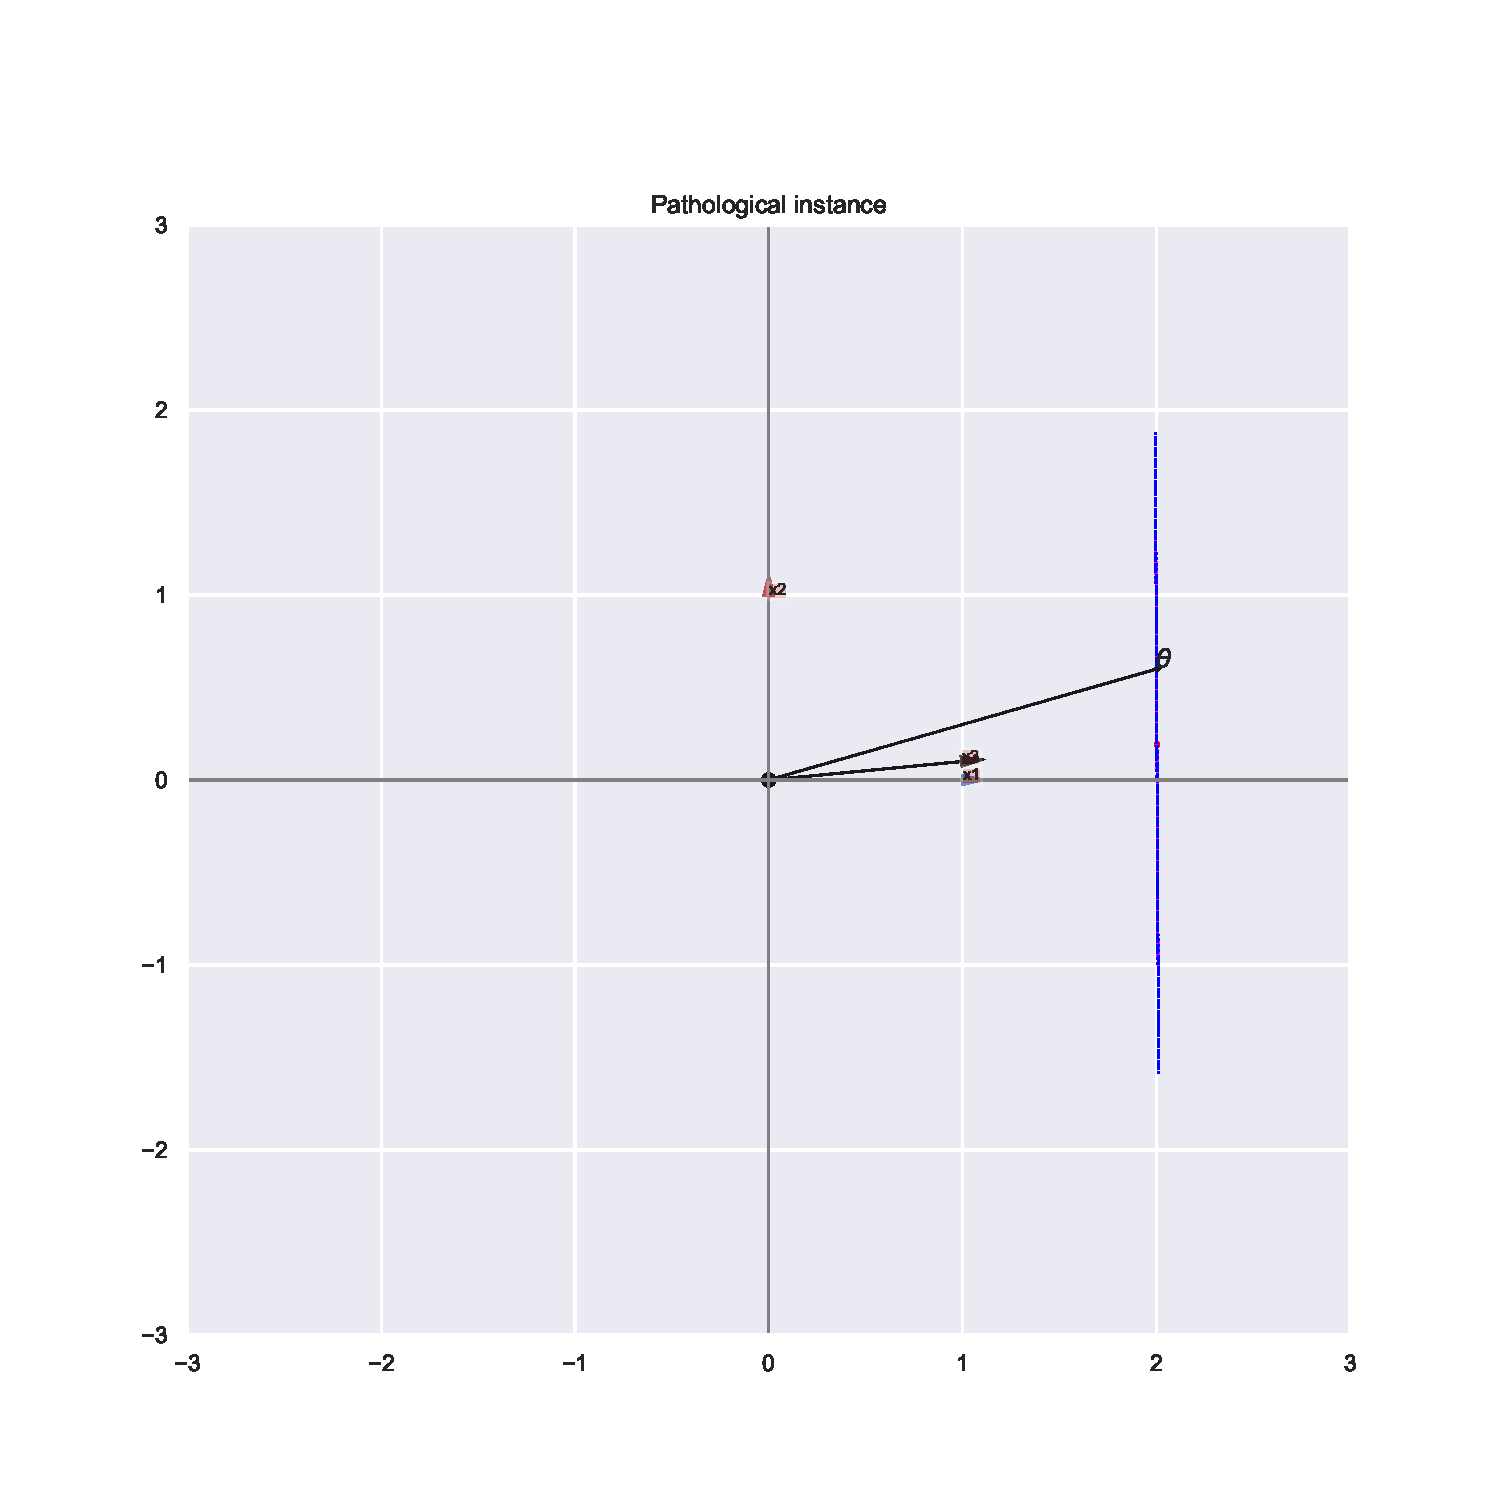
\includegraphics[width=0.55\textwidth]{Chapter4/img/instance.pdf}
    \caption{A pathological instance}
    \label{fig:instance}
\end{figure}
 =
\subsection{A "greedy" fix of \LTCC{}}

In order to overcome the previous issue, one can think of the following greedy version of $\LTCC$. It is inspired by the Greedy rule already used in (a heuristic version of) \LGapE~\citep{xu2018linear}, and is motivated by the following observation: in order to learn to discriminate between some arm $I^{(1)}$ and a challenger $I^{(2)}$, it may be more informative to select another arm. More specifically, the arm from which a new pull would reduce the most the variance in the estimation of $\bx_{I^{(1)}} - \bx_{I^{(2)}}$. In a standard bandit, this is simply the least pulled arm between $I^{(1)}$ and $I^{(2)}$, but in the linear case it may be another arm! 

\begin{algorithm}[ht]
\centering
\caption{Sampling rule (\LTCCG)}
\label{alg:lt3cg}
%\footnotesize
\begin{algorithmic}[1]
    %(and the $W_n$ function for \textcolor{red}{\TCC})
   %\STATE {\bfseries Initialization:} $\forall \blambda\in\Omega, S_{\blambda}=0, F_{\blambda}=0$
   \For{$n \leftarrow 1,2,\cdots$}
        \State \texttt{sample} $\btheta \sim \Pi_n$
        \State $\hat{\bx}^{(1)} \leftarrow \argmax_{\bx\in\cX} \bx\transpose\btheta$ \text{(indexed by $I^{(1)}$)}
	        \State $I^{(2)} \leftarrow \argmin_{i\neq I^{(1)}}W_n(I^{(1)},i)$ \text{(see \eqref{def:transportation} for the definition)}\Comment{$I^{(2)} \leftarrow \hat{\bx}^{(2)}$}
		    \State \texttt{evaluate arm} $\hat{\bx} \eqdef \argmin_{\bx\in\cX} \normm{\hat{\bx}^{(1)} - \hat{\bx}^{(2)}}_{(\bA_{\bX_n}+\bx\bx\transpose)^{-1}}$
	    \State \texttt{update mean and variance according to \eqref{eq:update_mean} and \eqref{eq:update_variance}}
	    \State $n = n+1$
   \EndFor
\end{algorithmic}
\end{algorithm}

\subsection{\texorpdfstring{\LGapE}{} versus \texorpdfstring{\LTCCG}{}: Is one of them optimal?}

Upon close examination, \LGapE and \LTCCG are very similar: they both rely on the computation of a leader and a challenger followed by the greedy rule to decide which arm to explore/play, and they actually use the same stopping rule (up to possible tuning of the threshold). The differences are:
\begin{itemize}
    \item how they define the challenger once the leader is chosen 
    \item how they perform exploration: \LGapE performs exploration in the choice of the challenger, which depends on some confidence bounds.  \LTCCG performs exploration in the choice of the leader, which is determined by Thompson sampling.  
\end{itemize}
An interesting direction of work is to know whether either of these algorithms is actually optimal:
\begin{itemize}
    \item for classical bandits (where \LTCCG can be seen as a "fix" of Best Challenger using Thompson sampling for leader selection, and playing the least drawn of the leader and challenger) 
    \item for linear bandits (in that case we will need to be able to actually compute the complexity and optimal weights efficiently to know if we are optimal!)
\end{itemize}

\medskip

Table~\ref{tab:comparison} provides a more detailed comparison of the two algorithms for linear bandits. We see in particular that the stopping rule coincide up to the choice $C_n = \sqrt{2\beta(n, \delta)}$.


\begin{table}[ht]
\centering
    %\hspace{-1cm}
    \resizebox{\textwidth}{!}{%
    \begin{tabular}{|c|c|c|}
    \hline 
      &  \LGapE & \LTCCG  \\
      \hline 
      Leader & $I_n^{(1)} = \argmax_{i}\bx_i\transpose\hat{\btheta}_n^{\lambda}$   &   $I_n^{(1)} = \argmax_{i} \bx_i\transpose\tilde{\btheta}_n$ \\
      & with $\hat \btheta_n^{\lambda}$ the least square estimate & with $\tilde{\btheta}_n \sim \mathcal{N}(\hat \btheta_n^\lambda,\hat{\bSigma}_n)$ \\
      \hline
        Challenger & $I_n^{(2)} = \underset{j \neq I_n^{(1)} }{\argmax} \ \left(\bx_j - \bx_{I_n^{(1)}}\right)\transpose \hat{\btheta}_n^\lambda + \normm{\bx_j - \bx_{I_n^{(1)}}}_{\hat{\bSigma}_n} C_n$    &   $I_n^{(2)} = \underset{j \neq I_n^{(1)} }{\argmin} \ddfrac{\left( \left(\bx_j - \bx_{I_n^{(1)}}\right)\transpose \hat\btheta_n^\lambda\right)^2}{2\normm{\bx_j - \bx_{I_n^{(1)}}}_{\hat{\bSigma}_n}^2} \1\left\{\bx_{I_n^{(1)}}\transpose\hat\btheta_n^\lambda \geq \bx_{j}\transpose\hat\btheta_n^\lambda\right\}$ \\
      \hline
          Stopping & $ \left(\bx_{I_n^{(2)}} - \bx_{I_n^{(1)}}\right)\transpose \hat\btheta_n^\lambda + \normm{\bx_{I_n^{(2)}} - \bx_{I_n^{(1)}}}_{\hat\bSigma_n} C_n < 0$    &  $\underset{j \neq J_n^{(1)} }{\min} \ddfrac{\left( \left(\bx_j - \bx_{J_n^{(1)}}\right)\transpose \hat\btheta_n^\lambda\right)^2}{2\normm{\bx_j - \bx_{J_n^{(1)}}}_{\hat{\bSigma}_n}^2} \1\left\{\bx_{J_n^{(1)}}\transpose\hat\btheta_n^\lambda \geq \bx_{j}\transpose\hat\btheta_n^\lambda\right\} > \beta(n,\delta)$ \\
                 & $ \Leftrightarrow \ddfrac{\left(\left(\bx_{I_n^{(1)}} - \bx_{I_n^{(2)}}\right)\transpose \hat\btheta_n^\lambda\right)^2}{2\normm{\bx_{I_n^{(2)}} - \bx_{I_n^{(1)}}}_{\hat\bSigma_n}^2} > C_n^2/2$    &   $\Leftrightarrow J_n^{(1)} = \argmax_{j} \bx_j\transpose\hat{\btheta}_n^\lambda, \ \ddfrac{\left(\left(\bx_{J_n^{(1)}} - \bx_{J_n^{(2)}}\right)\transpose \hat\btheta_n^\lambda\right)^2}{2\normm{\bx_{J_n^{(2)}} - \bx_{J_n^{(1)}}}_{\hat\bSigma_n}^2} > \beta(n,\delta)$ \\
          \hline
    \end{tabular}%
    }
\caption{Comparison between the two algorithms.} \label{tab:comparison}
\end{table}


% \subsection{Technical tools}

% \subsection{Tail bounds}
% Following are the classic Gaussian tail bound inequalities written in our linear context (see e.g.~\citealt{qin2017ttei} for detailed proofs).

% \begin{lemma}\label{lemma:tail_upper}
% For any $i,j\in\{1,\ldots,K\}$, if $\bx_i\transpose\hat{\btheta}^\lambda_n<\bx_j\transpose\hat{\btheta}^\lambda_n$,
% \begin{align}
%     \Pi_n\left[\bx_i\transpose\btheta>\bx_j\transpose\btheta\right] &\leq \frac{1}{2} \expp{-\frac{\left(\bx_j\transpose\hat{\btheta}^\lambda_n-\bx_i\transpose\hat{\btheta}^\lambda_n \right)^2}{2\normm{\bx_i-\bx_j}_{\hat{\bSigma}_n}^2}}.
% \end{align}
% \end{lemma}

% \begin{lemma}\label{lemma:tail_lower}
% For any $i,j\in\{1,\ldots,K\}$, if $\bx_i\transpose\hat{\btheta}^\lambda_n<\bx_j\transpose\hat{\btheta}^\lambda_n$,
% \begin{align}
%     \Pi_n\left[\bx_i\transpose\btheta>\bx_j\transpose\btheta\right] &\geq \frac{1}{\sqrt{2\pi}} \expp{-\frac{\left(\bx_j\transpose\hat{\btheta}^\lambda_n-\bx_i\transpose\hat{\btheta}^\lambda_n +\normm{\bx_i-\bx_j}_{\hat{\bSigma}_n}\right)^2}{2\normm{\bx_i-\bx_j}_{\hat{\bSigma}_n}^2}}.
% \end{align}
% \end{lemma}
